\documentclass{standalone}
\usepackage{tikz}

\begin{document}

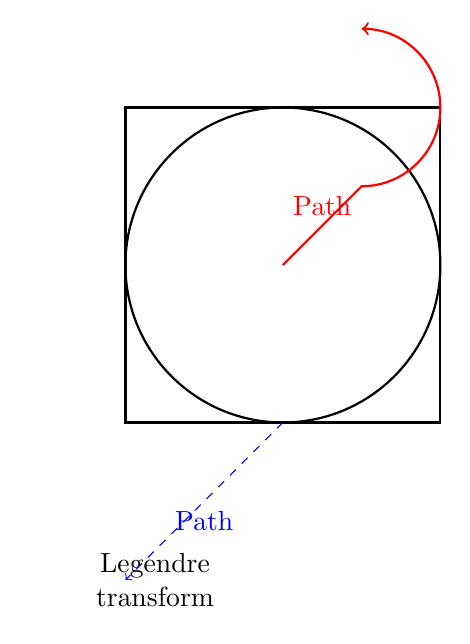
\begin{tikzpicture}[scale=2]

% Define the sectors
\draw[thick] (0,0) circle (1); % Positive sector
\draw[thick] (-1,-1) rectangle (1,1); % Negative sector

% Midpoints of the sectors
\coordinate (mid_pos) at (0,0);
\coordinate (mid_neg) at (0,0);

% Draw the path connecting the midpoints
\draw[->, thick, red] (mid_pos) -- node[midway, above] {Path} ++(0.5,0.5) arc[start angle=-90, end angle=90, radius=0.5];

% Left-hand side path indication
\node[left, text width=3cm, align=center] at (0,-2) {Legendre transform};
\draw[dashed, ->, blue] (0,-1) -- node[midway, below] {Path} ++(-1,-1);

\end{tikzpicture}

\end{document}